\documentclass{article}
\usepackage[utf8]{inputenc}
\usepackage[spanish]{babel}
\usepackage{listings}
\usepackage{url}
\usepackage{hyperref}
\usepackage{natbib}
\usepackage{graphicx}
\usepackage{color}

\title{Análisis de algoritmos: \\ Resolución al problema de la mochila 0-1.}
\author{Álvaro Antonio Soto Escobar \\ \href{mailto:asotoesc@itam.mx}{asotoesc@itam.mx} \\
CU: 160705}
\date{Septiembre 2016}

\begin{document}

\maketitle

\section{Introducción}
En algoritmia, el problema de la mochila, comúnmente abreviado por KP (del inglés Knapsack problem) es un problema de optimización combinatoria, es decir, que busca la mejor solución entre un conjunto finito de posibles soluciones a un problema. Modela una situación análoga al llenar una mochila, incapaz de soportar más de un peso determinado, con todo o parte de un conjunto de objetos, cada uno con un peso y valor específicos. Los objetos colocados en la mochila deben maximizar el valor total sin exceder el peso máximo.

\begin{figure}[h!]
    \centering
    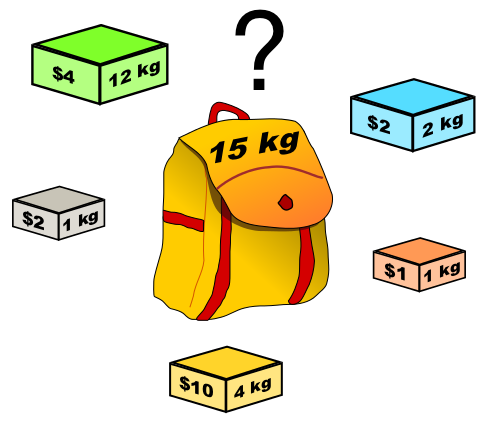
\includegraphics[scale=0.3]{img/Knapsack.png}
    \caption{Ejemplo del problema de la mochila}
    \label{fig:knapsack}
\end{figure}

\section{Definición del problema}
Supongamos que tenemos \textbf{n} distintos tipos de ítems, que van del \textbf{1} al \textbf{n} De cada tipo de ítem se tienen \(q_{i}\) ítems disponibles, donde \(q_{i}\) es un entero positivo.
Cada tipo de ítem \textit{i} tiene un \textbf{beneficio} asociado dado por \(v_{i}\) y un \textbf{peso} (o volumen) \(w_{i}\). Usualmente se asume que el beneficio y el peso no son negativos. Para simplificar la representación, se suele asumir que los ítems están listados en orden creciente según el peso (o volumen).
Por otro lado se tiene una mochila, donde se pueden introducir los ítems, que soporta un \textbf{peso máximo} (o volumen máximo) W.
El problema consiste en meter en la mochila ítems de tal forma que se \textbf{maximice el valor de los ítems que contiene y siempre que no se supere el peso (o volumen) máximo que puede soportar la misma}. La solución al problema vendrá dado por la secuencia de variables \(x_{1}\), \(x_{2}\), ..., \(x_{n}\) donde el valor de \(x_{i}\) indica cuantas copias se meterán en la mochila del tipo de ítem i.
\newline
El problema se puede expresar matemáticamente por medio del siguiente programa lineal:
\newline

{\displaystyle {\begin{array}{rl}{\text{maximizar }}&\sum _{i=1}^{n}v_{i}x_{i}\\{\text{tal que }}&\sum _{i=1}^{n}w_{i}x_{i}\leq W\\{\text{y}}&1\leq q_{i}\leq \infty .\end{array}}}

\vspace{5mm}
Si \(q_{i}\)=1 para i=1,2,...,n se dice que se trata del problema de la mochila 0-1. Si uno o más \(q_{i}\) es infinito entonces se dice que se trata del problema de la mochila no acotado también llamado a veces problema de la mochila entera. En otro caso se dice que se trata del problema de la mochila acotado. [1]


\section{Solución}

\begin{framed}
\lstinputlisting[label=knapsack, style=customc]{../knapsack.c}
\end{framed}

\vspace{10mm}
\section{Salida de ejecución}
\begin{framed}
\begin{lstlisting}
alvaro@skyline.headup.local:
hist:540  jobs:0 $ gcc knapsack.c  -o knapsack
alvaro@skyline.headup.local:
hist:541  jobs:0 $ ./knapsack 
Optimal value => 143
\end{lstlisting}
\end{framed}

\vspace{10mm}
\section{Referencias}

\begin{enumerate}
  \item \href{https://en.wikipedia.org/wiki/Knapsack_problem}{https://en.wikipedia.org/wiki/Knapsack\_problem} 
  \item \href{http://www.es.ele.tue.nl/education/5MC10/Solutions/knapsack.pdf}{http://www.es.ele.tue.nl/education/5MC10/Solutions/knapsack.pdf} 
  \item \href{https://www.youtube.com/watch?v=8LusJS5-AGo}{https://www.youtube.com/watch?v=8LusJS5-AGo} 
\end{enumerate}

\end{document}

